\chapter{Energy-Aware Gossip Protocol}
\label{Chapter3}
\lhead{Chapter 3. \emph{Energy-aware Gossip Protocol}} % Write in your own chapter title to set the page header

In this chapter, we will first introduce the classic \gp ~which will serve as a base protocol for other variations of gossip protocols. Then we will explain the detail of our basic push-pull \gp. And lastly, we will introduce our proposed energy-aware gossip protocol which is built based on the basic push-pull \gp.

\section{Classic Gossip Protocol}
% how gossip protocol works
\subsection{How It Works} \label{basic gossip}

The objective of gossip protocol is to broadcast messages in an efficient manner by mimicking social activities when people spread rumors in office by gossiping among each other. The classic \gp ~works as follows: when a node had a new message, it will send it to multiple randomly picked nodes in the network. Every node that received the new messages then will each randomly select multiple nodes and share the message with them. After a couple rounds of gossiping, majority of the nodes in the network have received this new message. The number of nodes a node tried to contacted is defined as the \emph{Fanout} of \gp. It is denoted as $f$. Each time when a node face the decision of whether sending a new message to another node or not, the probability of doing so is defined as $p_{gossip}$. In the rest of this thesis, I will refer to \emph{\pog} as $p_g$. Once a node received a new message, the number of times it will contact other nodes is defined as the \emph{Message Live Time} of \gp. It is denoted as $T_l$.

In a wired network setting , the \emph{\pog} of classic \gp ~is set to be 1 and \emph{Fanout} is usually set to be 1 or 2. \emph{Message Live Time} could vary depending on the application requirement. In a wireless ad-hoc network setting, a simple broadcasting by flooding would cause \emph{broadcast storm} problem \cite{tseng2002broadcast}. Due to overlapping radio signals in a geographical area, flooding often cause excessive redundancy, serious contention, and collision. Instead \emph{Fanout} is set to be 1 or 2 as well. However, people often tweak \emph{\pog} based on local or global network information such as total number of nodes, or node's degree (number of neighbors). Their goal is to reduce protocol overhead by lowering \emph{\pog} while still achieving decent message broadcasting coverage. 

%\subsection{Mathematical Model of Gossip Protocol}

\subsection{Key Gossip Protocol Control Parameters}
Four key parameters that define the behavior of gossip protocol in a wireless ad hoc network are: 

\begin{itemize}
	\item \emph{\pog}: $p_g  \quad (0 < p_g \leq 1)$
	\item \emph{Fanout}: $f = 1, 2, 3, \ldots$
	\item \emph{Message Live Time}: $T_l = 1,2,3, \ldots$
	\item \emph{Gossip Interval} $\Delta T_g$ (applicable when $T_l > 1$)
\end{itemize}

When $p_g = 1$ and $f = \mbox{node's degree}$, this protocol is closely resemble to flooding broadcast scheme which is not suitable for wireless ad hoc network. When $p_g = 1$ and $f = 1 \mbox{ or } 2$, this protocol is set to be classic \gp. $T_l$ is a parameter that is closely related to a node's memory constrain. A large $T_l$ setting will increase the message broadcasting successful rate at the expense of higher memory requirement and greater protocol overhead. 

\subsection{Variations of Gossip Protocol}

It is more clear when we category different variations of \gp ~into a matrix as shown in Table \ref{table:matrix}. 

\begin{table}[h]
	\centering
	\caption{Gossip Protocol Category Matrix}
	\label{table:matrix}
	\centering
	\begin{tabular}{|c|c|c|}
		\hline 
		& Global Network Information & Local Network Information \\ 
		\hline 
		Fixed  $p_g$ & \textbf{Quadrant I} & \textbf{Quadrant II} \\ 
		\hline 
		Adaptive $p_g$ & \textbf{Quadrant III} & \textbf{Quadrant IV} \\ 
		\hline 
	\end{tabular} 
\end{table}

The \emph{\pog} can be set to a fixed value or be adaptive. The basis of calculating $p_g$ can either be local network information such as node's degree (number of neighbors) or global network information such as number of nodes in the network. Therefore, we have four quadrants in this matrix. 

\begin{itemize}
	\item \textbf{Quadrant I}: fixed $p_g$ based on global network information. 
	\item \textbf{Quadrant II}: fixed $p_g$ based on local network information. 
	\item \textbf{Quadrant III}: adaptive $p_g$ based on global network information. 
	\item \textbf{Quadrant IV}: adaptive $p_g$ based on local network information. 
\end{itemize}

One observation is that researchers mainly focused on adjusting \emph{\pog}. Very little attention has been paid to another \gp ~parameter \emph{Fanout}. Fixed \emph{\pog} approaches can calculate its probability based on network density, distance among nodes, and speed \cite{2015survey}. In this scheme, nodes forward an incoming message with a fixed $p_g$, and the probability of not forwarding the incoming packet is $(1-p_g)$ \cite{2015survey}. The major challenge of fixed scheme is determining the optimal $p_g$. Due to the dynamic nature of wireless ad-hoc network, even an optimal initial global $p_g$ could become sub-optimal overtime. 

Adaptive \emph{\pog} approaches uses local or global network information such as density and speed to adjust individual or global probability. In adaptive scheme, there are adaptive non-counter-based schemes and adaptive counter-based schemes \cite{2015survey}. Adaptive density-based schemes usually utilize node's degree metrics. In (nb-scheme) the $p_g$ has an inverse relationship with the number of neighbors of a node \cite{cartigny2003border}. If we denote node's degree as $n_b$, then 

\[ p_g = \frac{k}{n_b} \mbox{\quad where $k$ is the propagation factor}\]

The $k$ is used so that the maximum and minimum probability can be adjusted \cite{cartigny2003border}. The basic idea behind this approach is that for a node with higher node's degree (meaning it has more neighbors, thus this area is more dense), a lower \emph{\pog} will be sufficient to spread out the new message. While for an sparse area, higher \emph{\pog} would be more desirable. Some paper \cite{qing2010dynamic}\cite{wisitpongphan2007broadcast} suggested schemes that dynamically adjust \emph{\pog} based on Received Signal Strength (RSS) or euclidean distance. In \cite{wisitpongphan2007broadcast}, the authors denoted the relative distance between node $i$ and node $j$ by $D_{ij}$ and the average transmission range by $r$. The \emph{\pog} is calculated using the following equation:

\[ p_g = \frac{D_{ij}}{r}\]

For a given $D_{ij}$, wider average transmission range will result in a lower \emph{\pog}. On the other hand, for a given average transmission range, \emph{\pog} will increase when the distance between node $i$ and node $j$ gets greater.

In counter-based schemes, nodes keep track with number of received copies of a given broadcast message and use it to determine its broadcasting state \cite{2015survey}. Similar to non-counter-density-based schemes, some paper \cite{lee2010adaptive} used node's degree in conjunction with a counter. The equation used to calculate \emph{\pog} is as follows:

\[ p_g = \frac{p_i}{n_b} \quad \mbox{where } p_i \mbox{ is the initial \pog}\]

The initial probability is set to be 1. If we denote the copy of messages threshold by $m_{th}$ and number of received copies of a given broadcast message by $m_r$, then whenever $m_r \geq m_{th}$, the above equation starts to kick in.

Similar to non-counter-distance-based schemes, some paper \cite{khan2008distance}\cite{ling2005coverage} used the distance between nodes as a metrics combining with a counter to determine the broadcasting state a node should be in. 

\section{Our Basic Push-Pull Gossip Protocol} \label{pp}
When each node in the network only forward new broadcast messages when it receive one, it is called a \emph{push} \gp. Similarly, when each node only request for new broadcast messages from other nodes, it is called  a \emph{pull} \gp. Our \gp combined both mechanisms thus it is called a \emph{push-pull} \gp. 

Our basic push-pull \gp ~utilizes three packet types to perform. They are:
\begin{itemize}
	\item Data packet
	\item Ack packet 
	\item Request packet
\end{itemize}

Data packet carries the actually payload (broadcast \msg). Ack packet and Request packet are used to control gossip process.There are several rules in our push-pull \gp. The Ack packet is used to acknowledge to the sender that receiver node already received that \msg ~before. The Request packet is used for a node to ask for the latest message from another node.

\begin{itemize}
	\item Rule 1: A node can only be in two states -- sleep state, and gossip state.
	\item Rule 2: Periodically, a node will request for a new \msg ~from one randomly selected neighbor regardless of its state.
	\item Rule 3: When a node received a new broadcast \msg, it will enter the gossip state.
	\item Rule 4: When a node is in gossip state, it will periodically randomly select $min(f, n_b)$ neighbors and forward the \msg ~to them.
	\item Rule 5: When a node received an Ack packet from any of its neighbor, it will enter sleep state which mean it will stop gossiping the new \msg.
	\item Rule 6: When a node received a duplicate \msg ~from anther node, it will send an Ack packet back. 
\end{itemize}

\begin{figure}[!htbp]
	\centering
	\begin{Verbatim}[fontsize=\small]
	
	// Periodic request 
	if state == gossip or state == sleep:
		every 5 seconds:
			find a random neighbor N
			send a Request packet to N
	
	// Periodic gossip	
	if state == gossip:
		every 1 second:
			find min(f, node's degree) random neighbors N<vector>
			send Data packet to N<vector>
	
	if state == sleep:
		Do nothing
	
	// Handle packets
	if receive a Data packet:
		if it is a new one:
			store the message
			state <- gossip
		else
			send an Ack back
	if received an Ack packet:
		state <- sleep
	if received a Request packet:
		send the latest message back	
	\end{Verbatim}
	\caption{The pseudo code of our push-pull \gp}
	\label{fig:pseudo}
\end{figure}

The pseudo code of our push-pull \gp ~is given in Figure~\ref{fig:pseudo}. All nodes in the network follow the same rules described above. For the sake of discussion, we assume that $f=1$ and there is no isolated node in the network. In the background, every node in the network will run a request process every 5 seconds regardless of its state. During the request process, it will randomly select a neighbor and request it to send its latest \msg. Initially, every node is in sleep state. Now let's assume that a new broadcast \msg ~is generated by node 1. Then node 1 immediately switch from sleep state to gossip state and start sending out this \msg ~to one of its neighbors. This gossip process runs every 5 seconds unless the node switched to sleep state. When a node switched to sleep state, it will do nothing. Now when a node received a Data packet, it will check for duplication. If it is indeed a new \msg, it will store the \msg ~and switch to gossip state. If it is not a new \msg, it will send an Ack packet back to the sender. If a node received an Ack packet, it will switch to sleep state. Lastly, if a node received a Request packet, it will send its latest \msg ~back to the sender. 

\section{Proposed Energy-Aware Adaptive Gossip Protocol}
As we stated previously in the thesis, the current state of research on gossip techniques for wireless broadcasting focused very little on energy efficiency and network lifetime. Far too many researches focused on dynamically adjusting $p_g$ based on global or local network information (global: number of nodes, local: node's degree, overhearing). Our objective here is to develop a new energy-aware gossip protocol that could extend network lifetime while still achieving a fast and reliable broadcasting performance. The parameter that we focused on shifted from \emph{\pog} to \emph{Fanout}.

Our observation tells us that a higher \emph{Fanout} setting will result in a shorter broadcasting time for a new message at the expense of higher energy consumption. While a lower \emph{Fanout} setting conserves energy, it results in a longer broadcasting time. First of all, we argue that each node's battery life should be maximized in order to extend network lifetime. Since for a broadcasting protocol, any node that is disconnected from the network due to energy depletion renders a situation that broadcasting can no longer work. In order to maximize each node's battery life, a constant high \emph{Fanout} setting is undesirable when battery is very low. Similarly when battery is very high, a constant low \emph{Fanout} setting can hinder the message broadcasting time. Therefore, we proposed that \emph{Fanout} should be dynamically adjusted based on each node's remaining energy fraction. 

Let's denoted the \emph{Remaining Energy Fraction} as $E_{frac}$. The function that used to calculate \emph{Fanout} is defined as follow:

\begin{equation*}
	f = \left\{
	\begin{array}{rl}
		5 & \text{if } 0.8 \leq E_{frac} \leq 1,\\
		4 & \text{if } 0.6 \leq E_{frac} \leq 0.8,\\
		3 & \text{if } 0.4 \leq E_{frac} \leq 0.6,\\
		2 & \text{if } 0.2 \leq E_{frac} \leq 0.4,\\					
		1 & \text{if } 0.0 \leq E_{frac} \leq 0.2.
	\end{array} \right.
\end{equation*}

The function is plotted in Figure \ref{fig:step}.

\begin{figure}[h]
	\centering
	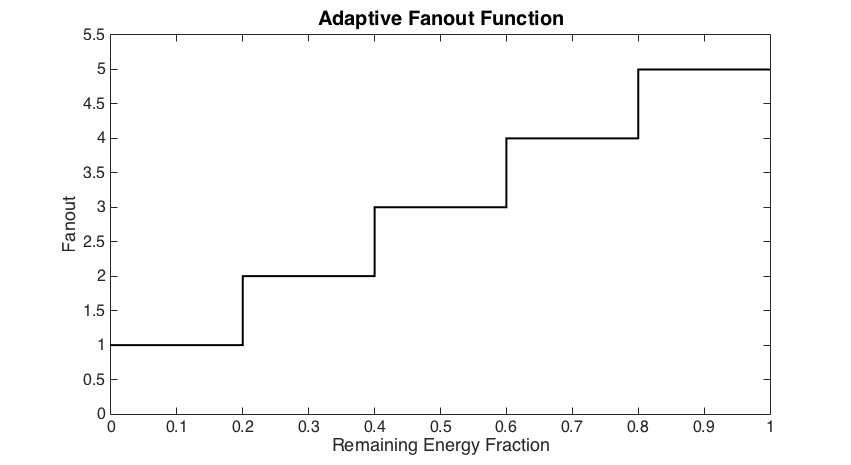
\includegraphics[width=5.5in]{stepFunction2.png}
	\caption{Adaptive fanout function plot}
	\label{fig:step}
\end{figure}

The basic idea of our fanout function is that the \emph{Fanout} of a node will gradually stepping down as its battery energy being drained. We believe this new fanout function can combine the advantages of both worlds. When a node's has plenty of energy left, it will reach out to more neighbors and facilitate \msg ~broadcasting process. As a node's energy gets lower, it will conserve its battery energy by contacting less neighbors thus extend network lifetime.

\begin{figure}[!htbp]
	\centering
	\begin{Verbatim}[fontsize=\small]	
	// Periodic gossip	
	if state == gossip:
		every 1 second:
			calculate the fanout f based on its energy fraction
			find min(f, node's degree) random neighbors N<vector>
			send Data packet to N<vector>
	\end{Verbatim}
	\caption{The pseudo code of our adaptive fanout push-pull \gp}
	\label{fig:gossip}
\end{figure}

Now we could tweak our basic push-pull \gp ~that we explained in Section \ref{pp} based on the proposed fanout function. The pseudo code of adaptive fanout push-pull \gp ~is given in Figure~\ref{fig:gossip}. Every time when a node tries to gossip a new \msg, it will first calculate the \emph{Fanout} using the adaptive fanout function. One thing that worth mentioning here is that \emph{Fanout} cannot exceed its node's degree. So here we have to take the minimum number between the calculated \emph{Fanout} and node's degree. For example, if a node only has 3 neighbors but the result from the fanout function is 5, the actual \emph{Fanout} will be 3.
